\chapter{Testování}\label{testovuxe1nuxed}

Pro účely testování bylo požádáno několik kolegů, aby zaujali pozici
testerů a~v~herně \emph{Virtualnirealita.cz} otestovali průběh výuky a
práci se spouštěčem.

Jelikož jde o~aplikaci s~lineárním postupem, nebyly k~testování
sestaveny scénáře ani průběhy. Testování tak proběhlo zjednodušeně, kdy
každý tester byl požádán, aby prošel výukou a~spustil VR~aplikaci dle
jeho výběru. V~průběhu jeho konání pak byl pozorován a~průběžně
byly zapisovány odchylky od očekávaného chování uživatele. Následně se 
položil malý počet kontrolních otázek.

\section{Předměty testování}\label{pux159edmux11bty-testovuxe1nuxed}

Z~funkčních požadavků definovaných v~analytické části byl stanoven
krátký seznam otázek, kterými se doplnilo testování:

\begin{itemize}
  \item
    Pochopili jste ovládání systému \emph{HTC Vive}?
  \item
    Chyběla vám ve výuce nějaká informace? Pokud by vás takto provázela osoba,
    zeptali byste se jí na nějakou otázku?
  \item
    Rozptylovalo vás při výuce něco?
  \item
    Byla pro vás výuka dostatečně svižná a~rychlá?
\end{itemize}
    
\section{Výsledky testování}\label{vysledky-testovani}

Na otázky testeři odpovídali pozitivně. Neshledali na průběhu výuky
žádnou vadu. Jeden z~testerů označil prostředí jako strohé, a~uvítal by,
kdyby bylo více rozmanité.

Jako věcnou připomínku lze také považovat názor přítomného kolegy, který se
neúčastnil testování. Konstatoval, že by se mu výuka líbila více, pokud by byla
pojata formou hry. Nelíbilo se mu, že jde o~strohou lineární instruktáž. Ač je
jeho názor čistě subjektivní, je to myšlenka, se kterou lze v~budoucnu pracovat.

Problémy byly shledány především v~technickém provedení. Aplikace 
byla nedostatečně odladěná, zpětná vazba testerů se skládala 
převážně z~chyb a~problémů, na které narazili.

Délka výuky byla o~něco vyšší, než očekávaná. Stále ji lze na základě analýzy označit
jako krátkou a~konstatovat, že splňuje stanovený požadavek \emph{N-04} na časovou efektivitu.

Délka výuky byla průměrně \textbf{2 minuty a~48 vteřin}.

\begin{figure}[h!]
\centering
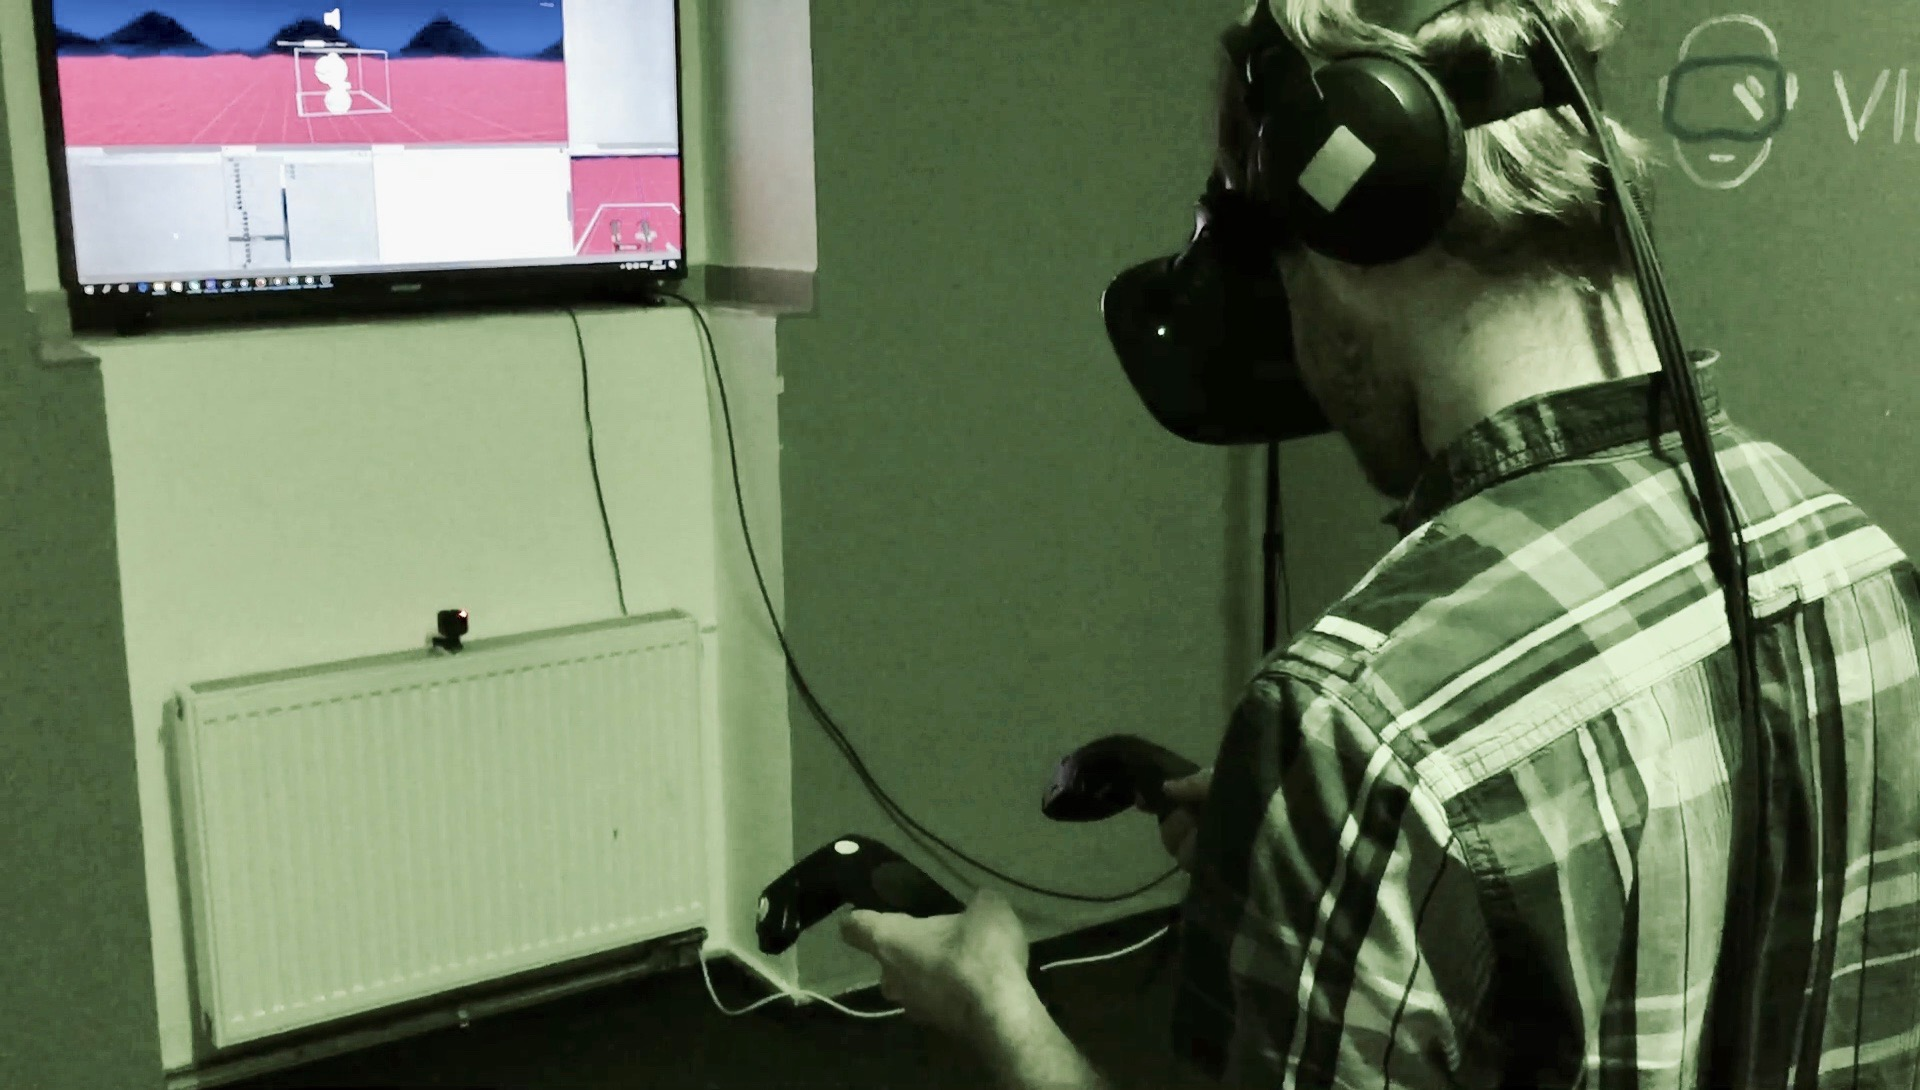
\includegraphics[width=12cm]{src/assets/testing.jpg}
\caption{Fotografie z~testování v~herně virtuální reality}
\end{figure}

\section{Zjištěné nedostatky a~jejich řešení}\label{zjiux161tux11bnuxe9-nedostatky}

Nedostatky v~aplikaci jsou převážně technické. Aplikace v~době testování trpěla na
chyby v~průběhu výuky a~vykreslování vizuálního prostředí.

Jako méně závažné lze označit chyby ve vykreslování. Určité prvky rozhraní se v~některých
chvílích překrývaly a~po skončení výuky byla stále zobrazena nápověda pro stisk
tlačítka, o~kterém bylo ve výuce naposledy hovořeno.

Větší problémy představovaly chyby, které přímo ovlivňovaly kvalitu 
výuky. Jednomu z~testerů nebylo umožněno stisknout tlačítko na výzvu 
výuky na jednom ze dvou ovladačů. Dalšímu z~testerů pak nefungoval 
barevný výběr laserového ukazovátka.

Všechny chyby byly zapsány a~budou před produkčním nasazením opraveny.

Testování lze označit jako úspěšné a~především užitečné. Odhalilo 
nespočet nedostatků a~pozorování chování napomohlo vzniku
několika dalších nápadů, jak aplikaci v~budoucnu vylepšit.